%package list
\documentclass{article}
\usepackage[top=3cm, bottom=3cm, outer=3cm, inner=3cm]{geometry}
\usepackage{multicol}
\usepackage{graphicx}
\usepackage{url}
%\usepackage{cite}
\usepackage{hyperref}
\usepackage{array}
%\usepackage{multicol}
\newcolumntype{x}[1]{>{\centering\arraybackslash\hspace{0pt}}p{#1}}
\usepackage{natbib}
\usepackage{pdfpages}
\usepackage{multirow}
\usepackage[normalem]{ulem}
\useunder{\uline}{\ul}{}
\usepackage{svg}
\usepackage{xcolor}
\usepackage{listings}
\lstdefinestyle{ascii-tree}{
    literate={├}{|}1 {─}{--}1 {└}{+}1 
  }
\lstset{basicstyle=\ttfamily,
  showstringspaces=false,
  commentstyle=\color{red},
  keywordstyle=\color{blue}
}
%\usepackage{booktabs}
\usepackage{caption}
\usepackage{subcaption}
\usepackage{float}
\usepackage{array}

\newcolumntype{M}[1]{>{\centering\arraybackslash}m{#1}}
\newcolumntype{N}{@{}m{0pt}@{}}


%%%%%%%%%%%%%%%%%%%%%%%%%%%%%%%%%%%%%%%%%%%%%%%%%%%%%%%%%%%%%%%%%%%%%%%%%%%%
%%%%%%%%%%%%%%%%%%%%%%%%%%%%%%%%%%%%%%%%%%%%%%%%%%%%%%%%%%%%%%%%%%%%%%%%%%%%
\newcommand{\itemEmail}{}
\newcommand{\itemStudent}{Milene Pacheco Esquinarila Isasi Vargas Angie}
\newcommand{\itemCourse}{Pweb2}
\newcommand{\itemSemester}{III}
\newcommand{\itemUniversity}{Universidad Nacional de San Agustín de Arequipa}
\newcommand{\itemFaculty}{Facultad de Ingeniería de Producción y Servicios}
\newcommand{\itemDepartment}{Departamento Académico de Ingeniería de Sistemas e Informática}
\newcommand{\itemSchool}{Escuela Profesional de Ingeniería de Sistemas}
\newcommand{\itemAcademic}{2024 - A}
\newcommand{\itemInput}{}
\newcommand{\itemOutput}{}
\newcommand{\itemPracticeNumber}{06}
\newcommand{\itemTheme}{DJango 1}
%%%%%%%%%%%%%%%%%%%%%%%%%%%%%%%%%%%%%%%%%%%%%%%%%%%%%%%%%%%%%%%%%%%%%%%%%%%%
%%%%%%%%%%%%%%%%%%%%%%%%%%%%%%%%%%%%%%%%%%%%%%%%%%%%%%%%%%%%%%%%%%%%%%%%%%%%

\usepackage[english,spanish]{babel}
\usepackage[utf8]{inputenc}
\AtBeginDocument{\selectlanguage{spanish}}
\renewcommand{\figurename}{Figura}
\renewcommand{\refname}{Referencias}
\renewcommand{\tablename}{Tabla} %esto no funciona cuando se usa babel
\AtBeginDocument{%
	\renewcommand\tablename{Tabla}
}

\usepackage{fancyhdr}
\pagestyle{fancy}
\fancyhf{}
\setlength{\headheight}{30pt}
\renewcommand{\headrulewidth}{1pt}
\renewcommand{\footrulewidth}{1pt}
\fancyhead[L]{\raisebox{-0.2\height}{
\includegraphics[width=3cm]{img/logo_episunsa.png}}}
\fancyhead[C]{\fontsize{7}{7}\selectfont	\itemUniversity \\ \itemFaculty \\ \itemDepartment \\ \itemSchool \\ \textbf{\itemCourse}}
\fancyhead[R]{\raisebox{-0.2\height}{
\includegraphics[width=1.2cm]{img/logo_abet}}}
\fancyfoot[L]{Estudiante Milene Pacheco Esquinarila}
\fancyfoot[C]{\itemCourse}
\fancyfoot[R]{Página \thepage}

% para el codigo fuente
\usepackage{listings}
\usepackage{color, colortbl}
\definecolor{dkgreen}{rgb}{0,0.6,0}
\definecolor{gray}{rgb}{0.5,0.5,0.5}
\definecolor{mauve}{rgb}{0.58,0,0.82}
\definecolor{codebackground}{rgb}{0.95, 0.95, 0.92}
\definecolor{tablebackground}{rgb}{0.8, 0, 0}

\lstset{frame=tb,
	language=bash,
	aboveskip=3mm,
	belowskip=3mm,
	showstringspaces=false,
	columns=flexible,
	basicstyle={\small\ttfamily},
	numbers=none,
	numberstyle=\tiny\color{gray},
	keywordstyle=\color{blue},
	commentstyle=\color{dkgreen},
	stringstyle=\color{mauve},
	breaklines=true,
	breakatwhitespace=true,
	tabsize=3,
	backgroundcolor= \color{codebackground},
}

\begin{document}

	
	\vspace*{10px}
	
	\begin{center}	
		\fontsize{17}{17} \textbf{ Informe de Laboratorio \itemPracticeNumber}
	\end{center}
	\centerline{\textbf{\Large Tema: \itemTheme}}
	%\vspace*{0.5cm}	

	\begin{flushright}
		\begin{tabular}{|M{2.5cm}|N|}
			\hline 
			\rowcolor{tablebackground}
			\color{white} \textbf{Nota}  \\
			\hline 
			     \\[30pt]
			\hline 			
		\end{tabular}
	\end{flushright}	

	\begin{table}[H]
		\begin{tabular}{|x{4.7cm}|x{4.8cm}|x{4.8cm}|}
			\hline 
			\rowcolor{tablebackground}
			\color{white} \textbf{Estudiante} & \color{white}\textbf{Escuela}  & \color{white}\textbf{Asignatura}   \\
			\hline 			{\itemStudent \par \itemEmail} & \itemSchool & {\itemCourse \par Semestre: \itemSemester \par}     \\
			\hline 			
		\end{tabular}
	\end{table}		
	
	\begin{table}[H]
		\begin{tabular}{|x{4.7cm}|x{4.8cm}|x{4.8cm}|}
			\hline 
			\rowcolor{tablebackground}
			\color{white}\textbf{Laboratorio} & \color{white}\textbf{Tema}  & \color{white}\textbf{Duración}   \\
			\hline 
			\itemPracticeNumber & \itemTheme &  horas   \\
			\hline 
		\end{tabular}
	\end{table}
	
	\begin{table}[H]
		\begin{tabular}{|x{4.7cm}|x{4.8cm}|x{4.8cm}|}
			\hline 
			\rowcolor{tablebackground}
			\color{white}\textbf{Semestre académico} & \color{white}\textbf{Fecha de inicio}  & \color{white}\textbf{Fecha de entrega}   \\
			\hline 
			\itemAcademic & \itemInput &  \itemOutput  \\
			\hline 
		\end{tabular}
	\end{table}
	 \\
  
	\section{Ejercicios Propuestos}
	\begin{itemize}		
  \\
 \item Implementa un Sistema en Django que maneje una tabla de Alumnos, una de Cursos y una de NotasAlumnosPorCurso y que permita ingresar a nuevos alumnos, nuevos cursos y finalmente permita ingresar las notas por curso.
Laboratorio realizado en grupos de 2 estudiantes.  Crear un unico proyecto y compartir github con el profesor (CarloCorrales010).
No olvidar enviar video a flipgrip de manera personal.


	\end{itemize}


 \\
  \\
 \section{URL de Repositorio Github}
	\begin{itemize}
		\item https://github.com/Milene-pe/LAB-PWEB2/tree/main/LAB06

	\end{itemize}

 \section{Código:}
     \item Directorio:
	\begin{figure}[H]
           \centering
           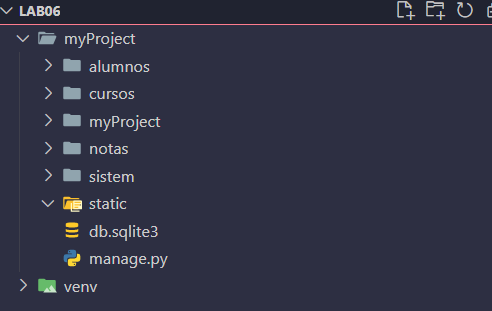
\includegraphics[scale=0.5]{latex/img/img1.png}
           %\includesvg{img/automata.svg}
           %\label{img:mot2}
           %\caption{Product backlog.}
     \end{figure}

\newpage

 \item Creamos nuestro entorno virtual:

    \begin{figure}[H]
           \centering
           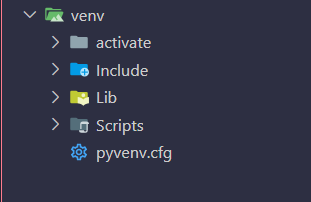
\includegraphics[scale=0.7]{latex/img/img2.png}
           %\includesvg{img/automata.svg}
           %\label{img:mot2}
           %\caption{Product backlog.}
     \end{figure}

 \item Esta tarea indica crear 3 aplicaciones, las cuales nombré como: alumnos, cursos y notas, para lo cual las agregue al settings.py de mi proyecto 
  
    \begin{figure}[H]
           \centering
           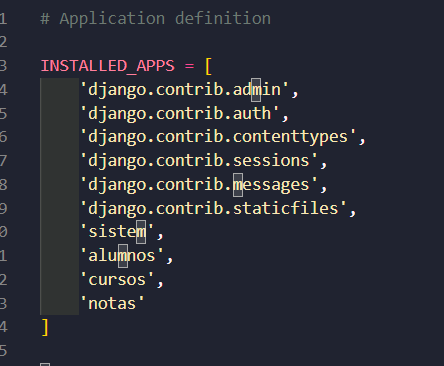
\includegraphics[scale=0.7]{latex/img/img4.png}
           %\includesvg{img/automata.svg}
           %\label{img:mot2}
           %\caption{Product backlog.}
     \end{figure}

 
\textbf{\large Aplicación Alumnos}
 \item    Se crean por defectos los archivos admin.py, apps.py, models.py, tests.py y view.py. 
 \item    Pero se creo el forms.py, se mostrará los cambios que se hizo en los archivos
  \item  Los datos que se solicitará serán nombres, apellidos y CUI
 
    \begin{figure}[H]
           \centering
           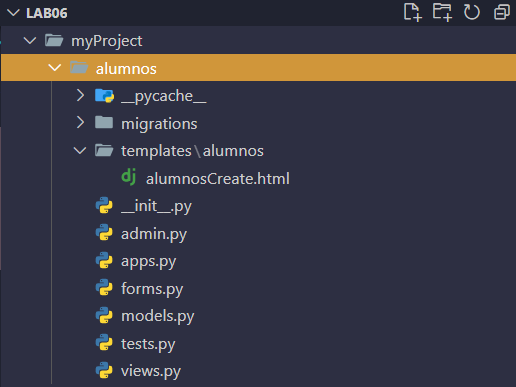
\includegraphics[scale=0.6]{latex/img/img3.png}
           %\includesvg{img/automata.svg}
           %\label{img:mot2}
           %\caption{Product backlog.}
     \end{figure}


\item admin.py:
 
\begin{lstlisting}
from django.contrib import admin
from .models import Alumno

admin.site.register(Alumno)

\end{lstlisting}

\item apps.py:
 
\begin{lstlisting}
from django.apps import AppConfig


class AlumnoConfig(AppConfig):
    default_auto_field = 'django.db.models.BigAutoField'
    name = 'alumnos'

\end{lstlisting}

\item models.py:
 
\begin{lstlisting}
from django.db import models

class Alumno(models.Model):
    nombre = models.CharField(max_length=100)
    apellido = models.CharField(max_length=100)
    cui = models.IntegerField()
   

\end{lstlisting}
     
\item  views.py:
 
\begin{lstlisting}
from django.shortcuts import render
from .models import Alumno
from .forms import AlumnoForm

# Create your views here.
def alumnoTestView(request):
    
    obj = Alumno.objects.get(id = 1)
    context = {
        'objecto':obj,
        }
    return render(request, 'alumnos/descripcion.html', context)
def alumnoCreateView(request):
    form = AlumnoForm(request.POST or None)
    if form.is_valid():
        form.save()
        form = AlumnoForm()
        
    
    return render(request, 'alumnos/alumnosCreate.html', {'form': form})

\end{lstlisting}
\newpage
 \item Se creo el forms.py ya que la tarea solicita que mediante un formulario se ingrese los datos y se guarden en  el panel de administracion de DJango:
	
\begin{lstlisting}
from django import forms

from .models import Alumno

class AlumnoForm(forms.ModelForm):
    class Meta:
        model = Alumno
        fields = [
            'nombre',
            'apellido',
            'cui',
        ]

\end{lstlisting}

 \item Se creo  alumnosCreate.html que conecta el formulario para poder ingresar los datos
 
\begin{lstlisting}
<!DOCTYPE html>
<html lang="en">
<head>
    <meta charset="UTF-8">
    <title>Crear Alumno</title>
</head>
<body>
    <header>
        <h1>Crear Alumno</h1>
    </header>
    <main>

        
        <form method="POST">
            
            {{ form.as_p }}
            <input type="submit" value="Grabar"/>
        </form>
        
    </main>
</body>
</html>

\end{lstlisting}

 \item Iniciaremos el servidor
 
     \begin{figure}[H]
           \centering
           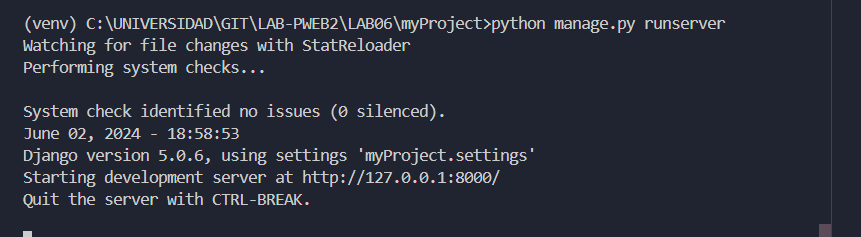
\includegraphics[scale=0.7]{latex/img/img5.png}
           %\includesvg{img/automata.svg}
           %\label{img:mot2}
           %\caption{Product backlog.}
     \end{figure}
     
 \item Vamos al http://127.0.0.1:8000/agregarAlumno/ y llenamos el formulario y verificamos si se guardo en el panel de DJango

     \begin{figure}[H]
           \centering
           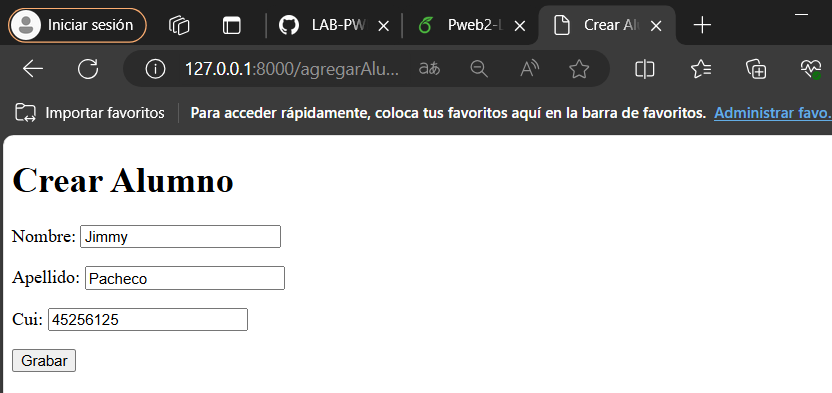
\includegraphics[scale=0.6]{latex/img/img6.png}
           %\includesvg{img/automata.svg}
           %\label{img:mot2}
           %\caption{Product backlog.}
     \end{figure}
     
 \item Verificamos en el panel de DJango

     \begin{figure}[H]
           \centering
           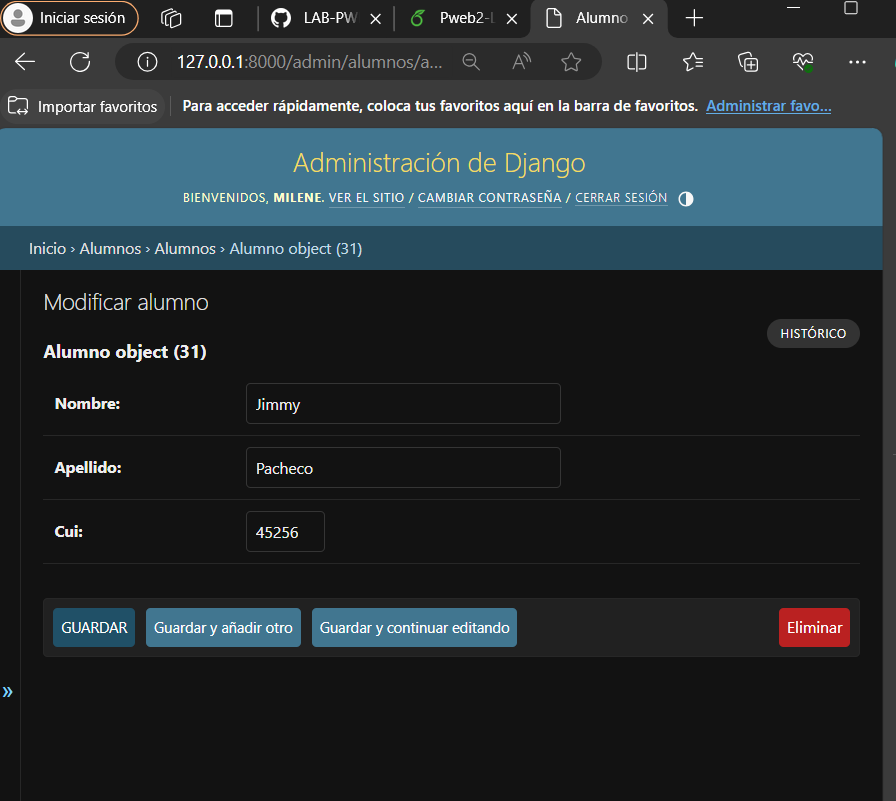
\includegraphics[scale=0.6]{latex/img/img7.png}
           %\includesvg{img/automata.svg}
           %\label{img:mot2}
           %\caption{Product backlog.}
     \end{figure}

     
\textbf{\large Aplicación Cursos}
 \item    Se crean por defectos los archivos admin.py, apps.py, models.py, tests.py y view.py. 
 \item    Pero se creo el forms.py, se mostrará los cambios que se hizo en los archivos
  \item  Los datos que se solicitará serán nombre, docente y codigo
 
    \begin{figure}[H]
           \centering
           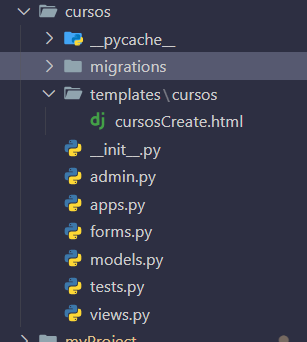
\includegraphics[scale=0.6]{latex/img/img8.png}
           %\includesvg{img/automata.svg}
           %\label{img:mot2}
           %\caption{Product backlog.}
     \end{figure}

\item admin.py:
 
\begin{lstlisting}
from django.contrib import admin
from .models import Curso

admin.site.register(Curso)

\end{lstlisting}

\item apps.py:
 
\begin{lstlisting}
from django.apps import AppConfig


class CursosConfig(AppConfig):
    default_auto_field = 'django.db.models.BigAutoField'
    name = 'cursos'
\end{lstlisting}

\item models.py:
 
\begin{lstlisting}
from django.db import models

class Curso(models.Model):
    nombre = models.CharField(max_length=100)
    docente = models.CharField(max_length=100)
    codigo = models.IntegerField()
   
\end{lstlisting}
     
\item  views.py:
 
\begin{lstlisting}
from django.shortcuts import render
from .models import Curso
from .forms import CursoForm

# Create your views here.
def cursoTestView(request):
    
    obj = Curso.objects.get(id = 1)
    context = {
        'objecto':obj,
        }
    return render(request, 'cursos/descripcion.html', context)
def cursoCreateView(request):
    form = CursoForm(request.POST or None)
    if form.is_valid():
        form.save()
        form = CursoForm()
        
    
    return render(request, 'cursos/cursosCreate.html', {'form': form})

\end{lstlisting}

 \item Se creo el forms.py ya que la tarea solicita que mediante un formulario se ingrese los datos y se guarden en  el panel de administracion de DJango:
	
\begin{lstlisting}
from django import forms

from .models import Curso

class CursoForm(forms.ModelForm):
    class Meta:
        model = Curso
        fields = [
            'nombre',
            'docente',
            'codigo',
            
        ]

\end{lstlisting}

 \item Se creo cursosCreate.html que conecta el formulario para poder ingresar los datos
 
\begin{lstlisting}
<!DOCTYPE html>
<html lang="en">
<head>
    <meta charset="UTF-8">
    <title>Crear Curso</title>
</head>
<body>
    <header>
        <h1>Crear Curso</h1>
    </header>
    <main>

        
        <form method="POST">
            
            {{ form.as_p }}
            <input type="submit" value="Grabar"/>
        </form>
        
    </main>
</body>
</html>


\end{lstlisting}

 \item Iniciaremos el servidor, e iremos al http://127.0.0.1:8000/agregarCurso/ y llenamos el formulario y verificamos si se guardo en el panel de DJango

     \begin{figure}[H]
           \centering
           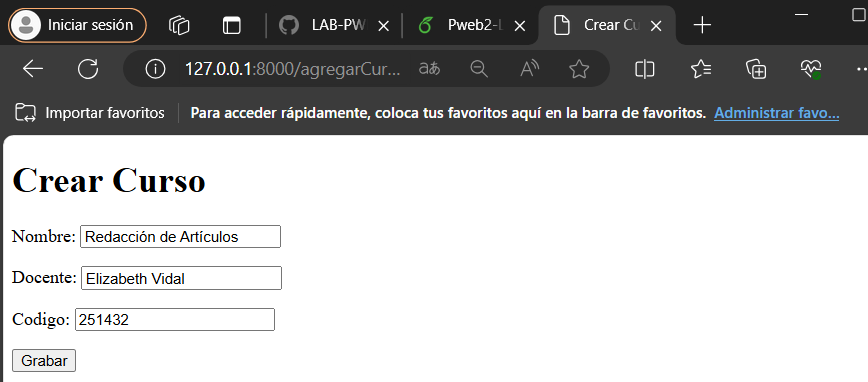
\includegraphics[scale=0.6]{latex/img/img9.png}
           %\includesvg{img/automata.svg}
           %\label{img:mot2}
           %\caption{Product backlog.}
     \end{figure}
     
 \item Verificamos en el panel de DJango

     \begin{figure}[H]
           \centering
           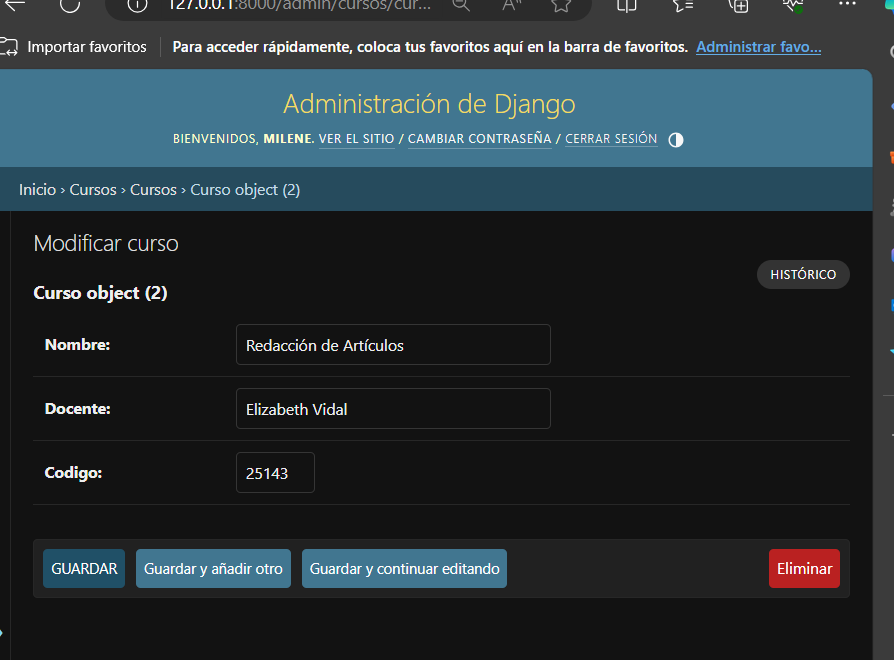
\includegraphics[scale=0.6]{latex/img/img10.png}
           %\includesvg{img/automata.svg}
           %\label{img:mot2}
           %\caption{Product backlog.}
     \end{figure}

\newpage
\textbf{\large Aplicación Notas}
 \item    Se crean por defectos los archivos admin.py, apps.py, models.py, tests.py y view.py. 
 \item    Pero se creo el forms.py, se mostrará los cambios que se hizo en los archivos
  \item  Los datos que se solicitará serán alumno, curso y nota
 
    \begin{figure}[H]
           \centering
           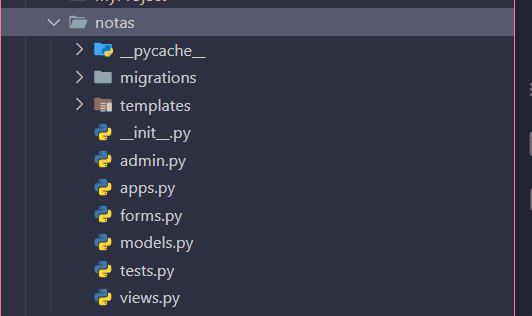
\includegraphics[scale=0.6]{latex/img/img11.png}
           %\includesvg{img/automata.svg}
           %\label{img:mot2}
           %\caption{Product backlog.}
     \end{figure}


\item admin.py:
 
\begin{lstlisting}
from django.contrib import admin
from .models import Nota

admin.site.register(Nota)

\end{lstlisting}

\item apps.py:
 
\begin{lstlisting}
from django.apps import AppConfig


class CursosConfig(AppConfig):
    default_auto_field = 'django.db.models.BigAutoField'
    name = 'notas'

\end{lstlisting}

\item models.py:
 
\begin{lstlisting}
from django.db import models

class Nota(models.Model):
    alumno = models.CharField(max_length=100)
    curso = models.CharField(max_length=100)
    nota = models.IntegerField()
   

\end{lstlisting}
     
\item  views.py:
 
\begin{lstlisting}
from django.shortcuts import render
from .models import Nota
from .forms import NotaForm

# Create your views here.
def notaTestView(request):
    
    obj = Nota.objects.get(id = 1)
    context = {
        'objecto':obj,
        }
    return render(request, 'notas/descripcion.html', context)
def notaCreateView(request):
    form = NotaForm(request.POST or None)
    if form.is_valid():
        form.save()
        form = NotaForm()
        
    
    return render(request, 'notas/notasCreate.html', {'form': form})

\end{lstlisting}

 \item Se creo el forms.py ya que la tarea solicita que mediante un formulario se ingrese los datos y se guarden en  el panel de administracion de DJango:
	
\begin{lstlisting}
from django import forms

from .models import Nota

class NotaForm(forms.ModelForm):
    class Meta:
        model = Nota
        fields = [
            'alumno',
            'curso',
            'nota',
            
        ]

\end{lstlisting}

 \item Se creo  notasCreate.html que conecta el formulario para poder ingresar los datos
 
\begin{lstlisting}
<!DOCTYPE html>
<html lang="en">
<head>
    <meta charset="UTF-8">
    <title>Crear Notas</title>
</head>
<body>
    <header>
        <h1>Crear Notas</h1>
    </header>
    <main>

        
        <form method="POST">
            
            {{ form.as_p }}
            <input type="submit" value="Grabar"/>
        </form>
        
    </main>
</body>
</html>


\end{lstlisting}

 \item Iniciaremos el servidor, e iremos al http://127.0.0.1:8000/agregarNota/ y llenamos el formulario y verificamos si se guardo en el panel de DJango

     \begin{figure}[H]
           \centering
           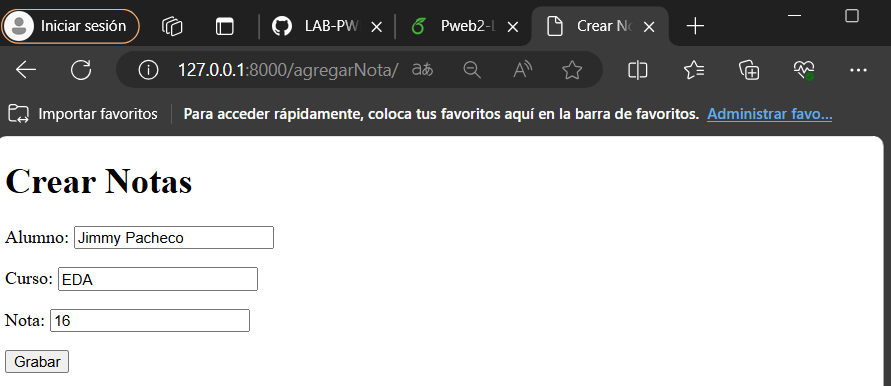
\includegraphics[scale=0.6]{latex/img/img12.png}
           %\includesvg{img/automata.svg}
           %\label{img:mot2}
           %\caption{Product backlog.}
     \end{figure}
     
 \item Verificamos en el panel de DJango

     \begin{figure}[H]
           \centering
           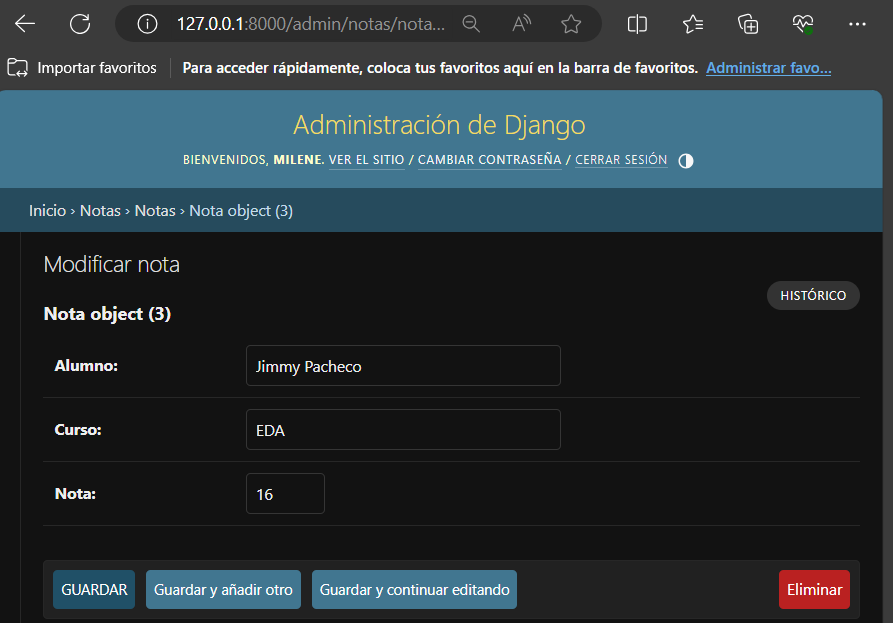
\includegraphics[scale=0.6]{latex/img/img13.png}
           %\includesvg{img/automata.svg}
           %\label{img:mot2}
           %\caption{Product backlog.}
     \end{figure}

     
\end{document}	

